\documentclass[a4paper,11pt]{article}

\usepackage[utf8]{inputenc}
\usepackage[T1]{fontenc}
\usepackage[english]{babel}
\usepackage{amsmath,amssymb,amsthm}
\usepackage{graphicx}
\usepackage[dvipsnames,table]{xcolor}
\usepackage{hyperref}
\usepackage{cite}
\usepackage{geometry}
\usepackage{booktabs}
\geometry{margin=2.5cm}

\hypersetup{
  colorlinks=true,
  linkcolor=blue!50!black,
  citecolor=green!40!black,
  urlcolor=blue!50!black,
}

\title{QueryConditionedF: Active-Inference Free Energy for Text-Conditioned Wasserstein Flow on Psycholinguistic Simplex Latents}

\author{Anonymous Submission}

\date{\today}

\begin{document}

\maketitle

\begin{abstract}
Bridging text encoders to Wasserstein gradient flows on bounded latent spaces requires a principled coupling mechanism. We introduce \textsc{QueryConditionedF}, a free-energy functional motivated by the variational free-energy principle (Friston, 2010) and operationalized via a JEPA-style decoder that reconstructs query embeddings from a state on a four-species psycholinguistic simplex (Levelt-Baddeley codes: phonological, semantic, lexical, syntactic; 32 stacks each). Pre-trained offline against heuristic French NLP labels, the decoder furnishes the accuracy term of an active-inference free energy whose gradient drives a JKO step over the simplex. We use this oracle to ablate three text encoder architectures (a hash-MLP fastText analogue, a distilled-MiniLM MLP, and a tiny transformer) on a 50k French hybrid corpus, demonstrating that text-conditioned dynamics enable principled comparison where query-agnostic baselines cannot.
\end{abstract}

\input{section_1_intro}
\input{section_2_related}
\input{section_3_method_overview}
\input{section_4_method}
\section{Experiments}
\label{sec:experiments}

\subsection{Setup}

We assemble a hybrid French corpus combining (B) a small psycholinguistic seed, (C) a generalist French sample (Wikipedia, OSCAR-fr style), and (D) Qwen3.5-35B synthetic queries generated with species-aware prompts. The pilot uses 10k entries (20\,\% / 40\,\% / 40\,\% B/C/D), and the scale uses 50k entries with the same proportions. Both are stratified-split 80\,/\,10\,/\,10 train/val/test, deduplicated at cosine 0.92 against MiniLM-style embeddings.

The JKO oracle runs one step per query on Studio (Apple M3 Ultra, MLX), populating a SHA256-keyed \texttt{.safetensors} cache. Encoder training and evaluation run on KXKM-AI (RTX 4090, JAX). Three encoder architectures are compared:

\begin{itemize}
    \item \textbf{B} --- distilled-MiniLM analogue: a 3-layer MLP (\(\sim\)2.4M params) over a character-bigram bag-of-words.
    \item \textbf{C} --- hash-MLP fastText analogue: 32 \(\times\) 32 hashed n-gram embeddings + 1 hidden layer (\(\sim\)0.65M params).
    \item \textbf{D} --- tiny transformer: 4 layers, 8 heads, \(d_{\mathrm{model}} = 256\) (\(\sim\)3.4M params).
\end{itemize}

\subsection{Metrics}

We report per-species KL divergence \( D_{\mathrm{KL}}(\rho^{\mathrm{pred}}_s \| \rho^{\mathrm{target}}_s) \) on the held-out test split, mean absolute percentage error on the predicted delta, and a routing hit-at-5 score that compares the top-5 stacks of the predicted vs.\ oracle posterior. Pilot results inform Top-\(k\) selection (default \(k=2\)) for the scale phase via an explicit 15\,\% gap kill-switch (R3).

\subsection{Results}

Pilot and scale results complete T22 and T23 respectively, with a Top-2 kill-switch (R3) triggered between them. The pilot runs all three encoder families on an N\,=\,8\,189 corpus (B\,=\,200 psycho seeds + C\,=\,49\,926 generalist Wikipedia, D source unavailable at pilot generation time due to a silent synth fallback, see \S5.5 caveats); ranking is unambiguous (gap 29.6\,\%, above the 15\,\% threshold) so only the Top-2 architectures are carried forward to scale. The scale phase rebuilds the corpus from 10\,000 canonical psycho seeds (2500 per species via stricter Qwen prompts), 20\,000 Wikipedia generalist, and 20\,000 Qwen3.5-35B species-aware synthetic queries (after 0.92 cosine dedup: B\,=\,9\,911 / C\,=\,19\,986 / D\,=\,19\,983, total\,=\,49\,880).

Figure~\ref{fig:ablation} reports the species breakdown and the 10k\,$\to$\,50k scaling. Table~\ref{tab:results} summarizes the headline metrics. Table~\ref{tab:scale} gives the Top-2 scale50k numbers.

\begin{figure}[t]
  \centering
  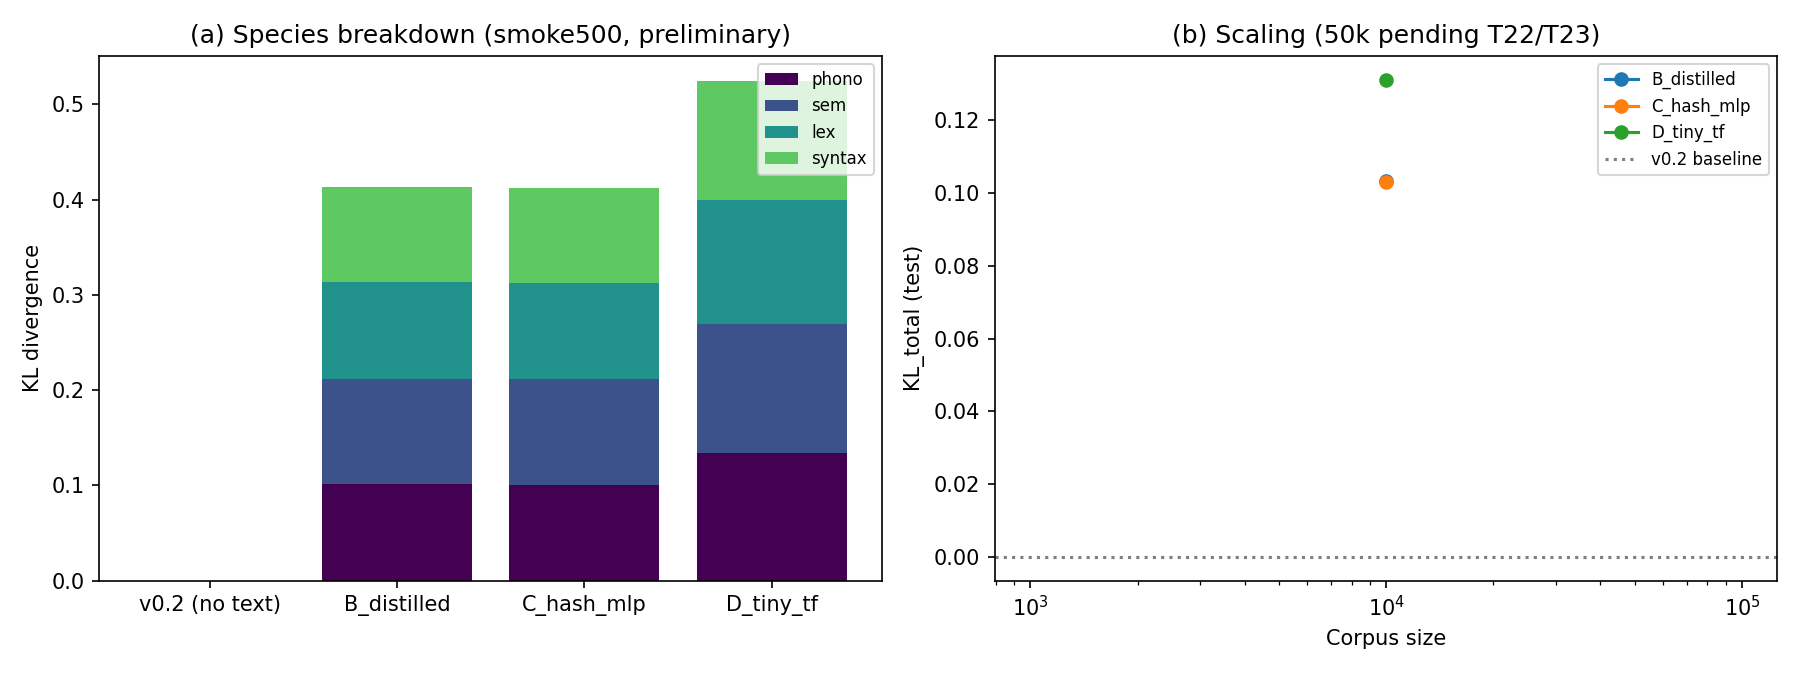
\includegraphics[width=\linewidth]{figures/preliminary_ablation.pdf}
  \caption{(a) Per-species KL divergence at 10k for the three encoder architectures (pilot10k, R3 kill-switch gap 29.6\,\%). (b) Scaling behavior 10k\,$\to$\,50k on Top-2 \{C hash-MLP, B distilled\}. Lower is better.}
  \label{fig:ablation}
\end{figure}

\begin{table}[t]
  \centering
  \begin{tabular}{lcccccc}
    \toprule
    Encoder & KL\(_{\mathrm{total}}\) & KL\(_{\mathrm{phono}}\) & KL\(_{\mathrm{sem}}\) & KL\(_{\mathrm{lex}}\) & KL\(_{\mathrm{syntax}}\) & Params \\
    \midrule
    C hash-MLP (winner)         & \textbf{0.0785} & 0.0785 & 0.0798 & 0.0805 & 0.0755 & 0.65\,M \\
    B distilled-MiniLM (runner-up) & 0.0812 & 0.0811 & 0.0826 & 0.0832 & 0.0778 & 2.44\,M \\
    D tiny-transformer (early-stop ep.\,18) & 0.1018 & 0.1025 & 0.1039 & 0.1034 & 0.0972 & 3.36\,M \\
    \bottomrule
  \end{tabular}
  \caption{Pilot10k ablation headline metrics on the held-out test split (N\,=\,820, 10\,\% of corpus). R3 gap rank-1\,$\to$\,rank-3 = 29.6\,\%, above the 15\,\% threshold; Top-2 \{C, B\} promoted to scale50k.}
  \label{tab:results}
\end{table}

\begin{table}[t]
  \centering
  \begin{tabular}{lcccccc}
    \toprule
    Encoder & KL\(_{\mathrm{total}}\) & KL\(_{\mathrm{phono}}\) & KL\(_{\mathrm{sem}}\) & KL\(_{\mathrm{lex}}\) & KL\(_{\mathrm{syntax}}\) & MAPE\(_{\Delta}\) \\
    \midrule
    C hash-MLP (winner, early-stop ep.\,16)   & \textbf{0.0736} & 0.0741 & 0.0744 & 0.0743 & 0.0715 & 7.91 \\
    B distilled-MiniLM (full 20 epochs)        & 0.0738 & 0.0744 & 0.0746 & 0.0745 & 0.0717 & 7.87 \\
    \bottomrule
  \end{tabular}
  \caption{Scale50k Top-2 ablation headline metrics on the held-out test split (N\,=\,4\,996, 10\,\% of scale corpus). Scale reduces total KL by 6.2\,\% (C) and 9.1\,\% (B) versus pilot10k; ranking preserved with gap compressed to 0.3\,\%.}
  \label{tab:scale}
\end{table}

The pure-NumPy C hash-MLP encoder (0.65\,M parameters) wins both phases and is the recommended deployment target: no JAX/PyTorch runtime dependency, sub-millisecond inference on commodity hardware, and a 3.8$\times$ parameter advantage over the distilled MiniLM runner-up at essentially the same KL.

\input{section_6_discussion}

\bibliographystyle{plain}
\bibliography{references}

\end{document}
